% Template inspired by Drew Ulick
% https://www.overleaf.com/articles/130-cheat-sheet/ntwtkmpxmgrp
\documentclass{article}
\usepackage[landscape]{geometry}
\usepackage{xifthen}
\usepackage{url}
\usepackage{tikz}
\usetikzlibrary{positioning,fit,calc,backgrounds}

\usepackage{xcolor}
\usepackage{enumitem}
\usepackage{amssymb, amsmath,endnotes}
\usepackage{multicol}
\usepackage{multirow}
\usepackage{fontawesome}
\usepackage{xparse}
\usepackage{listings}
\usepackage[utf8]{inputenc}
\usepackage[listings]{tcolorbox}
\tcbuselibrary{listings}
% \lstset{%
% basicstyle=\ttfamily,
% breaklines = true,
% backgroundcolor=\color{gray!30},
% }
\lstdefinestyle{simple}{ %
    basicstyle=\ttfamily,
    breaklines = true,
    backgroundcolor=\color{gray!30},
}
\lstdefinestyle{bash}{ %
  backgroundcolor=\color{gray!30},   % choose the background color; you must add \usepackage{color} or \usepackage{xcolor}; should come as last argument
  basicstyle=\ttfamily\footnotesize\color{black},        % the size of the fonts that are used for the code
  breakatwhitespace=false,         % sets if automatic breaks should only happen at whitespace
  breaklines=true,                 % sets automatic line breaking
  escapeinside={\%*}{*)},          % if you want to add LaTeX within your code
  extendedchars=true,              % lets you use non-ASCII characters; for 8-bits encodings only, does not work with UTF-8
  frame=single	                   % adds a frame around the code
  keepspaces=true,                 % keeps spaces in text, useful for keeping indentation of code (possibly needs columns=flexible)
  language=bash,                 % the language of the code
  keywordstyle=\bfseries,
  morekeywords={GET,POST,PUT,DELETE,... },           % if you want to add more keywords to the set
  numbers=left,                    % where to put the line-numbers; possible values are (none, left, right)
  numbersep=5pt,                   % how far the line-numbers are from the code
  numberstyle=\tiny\color{black}, % the style that is used for the line-numbers
  rulecolor=\color{black},         % if not set, the frame-color may be changed on line-breaks within not-black text (e.g. comments (green here))
  showspaces=false,                % show spaces everywhere adding particular underscores; it overrides 'showstringspaces'
  showstringspaces=false,          % underline spaces within strings only
  showtabs=false,                  % show tabs within strings adding particular underscores
  stepnumber=1,                    % the step between two line-numbers. If it's 1, each line will be numbered
  tabsize=2,	                   % sets default tabsize to 2 spaces
}
\lstdefinelanguage{json}{
    keywords={GET,POST,PUT,DELETE},
    keywordstyle=\color{darkgray!70!black}\bfseries,
    identifierstyle=\color{black},
    sensitive=false,
    comment=[l]{//},
    morecomment=[s]{/*}{*/},
    commentstyle=\color{purple}\ttfamily,
    stringstyle=\color{green!50!black}\ttfamily,
    morestring=[b]',
    morestring=[b]"
}
\lstdefinestyle{js}{ %
  backgroundcolor=\color{gray!30},   % choose the background color; you must add \usepackage{color} or \usepackage{xcolor}; should come as last argument
  basicstyle=\ttfamily\footnotesize\color{black},        % the size of the fonts that are used for the code
  breakatwhitespace=false,         % sets if automatic breaks should only happen at whitespace
  breaklines=true,                 % sets automatic line breaking
  escapeinside={\%*}{*)},          % if you want to add LaTeX within your code
  extendedchars=true,              % lets you use non-ASCII characters; for 8-bits encodings only, does not work with UTF-8
  frame=single	                   % adds a frame around the code
  keepspaces=true,                 % keeps spaces in text, useful for keeping indentation of code (possibly needs columns=flexible)
  language=json,                 % the language of the code
%   keywordstyle=\bfseries,
%   morekeywords={GET,POST,PUT,DELETE,... },           % if you want to add more keywords to the set
  numbers=left,                    % where to put the line-numbers; possible values are (none, left, right)
  numbersep=5pt,                   % how far the line-numbers are from the code
  numberstyle=\tiny\color{black}, % the style that is used for the line-numbers
  rulecolor=\color{black},         % if not set, the frame-color may be changed on line-breaks within not-black text (e.g. comments (green here))
  showspaces=false,                % show spaces everywhere adding particular underscores; it overrides 'showstringspaces'
  showstringspaces=false,          % underline spaces within strings only
  showtabs=false,                  % show tabs within strings adding particular underscores
  stepnumber=1,                    % the step between two line-numbers. If it's 1, each line will be numbered
  tabsize=2,	                   % sets default tabsize to 2 spaces
}
\lstset{style=simple}

\title{MISP Cheat Sheet}
\author{MISP Project}
\date{\today}

\makeatletter
\let\theauthor\@author
\let\thedate\@date
\makeatother
\advance\topmargin-.8in
\advance\textheight3in
\advance\textwidth3in
\advance\oddsidemargin-1.5in
\advance\evensidemargin-1.5in
\parindent0pt
\parskip2pt
\newcommand{\hr}{\centerline{\rule{3.5in}{1pt}}}
\newcommand{\events}{\texttt{Events }}
\newcommand{\event}{\texttt{Event }}
\newcommand{\attributes}{\texttt{Attributes }}
\newcommand{\attribute}{\texttt{Attribute }}
\newcommand{\objects}{\texttt{MISP Objects }}
\newcommand{\object}{\texttt{MISP Object }}
\newcommand{\reference}{\texttt{Reference }}
\newcommand{\references}{\texttt{References }}
\newcommand{\proposals}{\texttt{Proposals }}
\newcommand{\proposal}{\texttt{Proposal }}
\newcommand{\eventreports}{\texttt{Event Reports }}
\newcommand{\eventreport}{\texttt{Event Report }}
\newcommand{\sightings}{\texttt{Sightings }}
\newcommand{\sighting}{\texttt{Sighting }}
\newcommand{\taxonomies}{\texttt{Taxonomies }}
\newcommand{\taxonomy}{\texttt{Taxonomy }}
\newcommand{\galaxy}{\texttt{Galaxy }}
\newcommand{\galaxies}{\texttt{Galaxies }}
\newcommand{\clusters}{\texttt{Galaxy Clusters }}
\newcommand{\cluster}{\texttt{Galaxy Cluster }}
\newcommand{\sharinggroups}{\texttt{Sharing Groups }}
\newcommand{\sharinggroup}{\texttt{Sharing Group }}

\newcommand{\taggable}{\faicon{tags}\hspace*{0.3em}}
\newcommand{\distributable}{\faicon{eye-slash}\hspace*{0.3em}}
\newcommand{\synchronisable}{\faicon{exchange}\hspace*{0.3em}}
\tikzstyle{mybox} = [
    draw=black,
    fill=white,
    very thick,
    rectangle, rounded corners,
    inner sep=10pt, inner ysep=10pt
]
\tikzstyle{boxtitle} = [
    fill=black,
    text=white,
    font=\bfseries,
    right=10pt
]
% arg1 = icon
% arg2 = purpose
% arg3 = usecase
% arg4 = actions
% arg5 = description
% arg6 = title
% arg7 = content
\tikzset{actionbox/.style={
    text=white,
    yshift=-1pt,xshift=-1pt,
    append after command={
    \pgfextra
            \draw[sharp corners, fill=black]% 
        (\tikzlastnode.west)% 
        [rounded corners=0pt] |- (\tikzlastnode.north)% 
        [rounded corners] -| (\tikzlastnode.east)% 
        [rounded corners=0pt] |- (\tikzlastnode.south)% 
        [rounded corners] -| (\tikzlastnode.west);
    \endpgfextra
    }
}}
\NewDocumentCommand{\cheatbox}{ O{} O{} O{} O{} O{} m m}{
    \begin{tikzpicture}
        \node [mybox] (box){%
            \begin{minipage}{0.3\textwidth}
            \ifthenelse{\isempty{#4}}{}{\vspace{1em}}
            \textit{#5}
            \vspace*{0.3em}
            \ifthenelse{\isempty{#2}}{}{ \par{\textbf{Purpose}: #2}}
            \ifthenelse{\isempty{#3}}{}{ \par{\textbf{Usecase}: #3\ifthenelse{\isempty{#7}}{}{\\}}}
            #7
            \end{minipage}
        };
        \node[boxtitle] at (box.north west) {#1 #6};
        \ifthenelse{\isempty{#4}}{}{
            \path node [actionbox, anchor=north east] at (box.north east) (actionLabel) {#4};
        }
    \end{tikzpicture}

    \vspace*{2pt}
}
% arg1 = description
% arg2 = title
% arg3 = content
\newcommand{\cheatboxlarge}[3][]{
    \begin{tikzpicture}
        \node [mybox] (box){%
            \begin{minipage}{0.46\textwidth}
            \ifthenelse{\isempty{#1}}{}{\textit{#1}}
            \ifthenelse{\isempty{#1}}{}{\vspace{2pt}}
            #3
            \end{minipage}
        };
        \node[boxtitle] at (box.north west) {#2};
    \end{tikzpicture}

    \vspace*{3pt}
}
% arg1 = label
% arg2 = text
\newcommand{\boxentry}[2]{
    \par{\textbf{#1}: #2\vspace*{0.3em}}
}
% arg1 = label
% arg2 = text
\newcommand{\boxentrycompact}[2]{
    \par{\textbf{#1} #2}
}

% arg1 = current level
% arg2 = text
\newcommand{\changestyledistribution}[2]{
    % \ifthenelse{\isin{#1}{#2}}{
    \ifthenelse{#1 > #2}{
        \tikzset{currentstyle/.style=fullnode}
    }{
        \tikzset{currentstyle/.style=emptynode}
    }
}
% arg1 = label
% arg2 = text
\newcommand{\distrigraph}[1]{
    \def \scale {0.2}
    \begin{tikzpicture}[
        emptynode/.style={circle, draw=black, scale=\scale},
        fullnode/.style={circle, draw=black, fill=black, scale=\scale},
    ]
    \tikzset{
        currentstyle/.style={}
    }
        \changestyledistribution{#1}{0}
        \node[currentstyle] (d0)  {};
        \changestyledistribution{#1}{1}
        \node[currentstyle] (d1a) [above right= 1pt and 30pt of d0] {};
        \node[currentstyle] (d1b) [below right= 1pt and 30pt of d0] {};
        \changestyledistribution{#1}{2}
        \node[currentstyle]  (d2)  [right=of d1b] {};
        \changestyledistribution{#1}{2}
        \node[currentstyle]  (d3)  [right=of d2] {};

        \draw[-] (d0) to[out=30, in=180] (d1a);
        \draw[-] (d0) to[out=-30, in=180] (d1b);
        \draw[-] (d1b) -- (d2);
        \draw[-] (d2) -- (d3);
    \end{tikzpicture}
}

\begin{document}

\begin{center}{
    \huge{\textbf{MISP Concept Cheat sheet}}}\\
\end{center}
\begin{multicols*}{2}

\cheatboxlarge{Glossary}{

    \boxentry{Correlations}{Are links created automatically whenever an \attribute is created or modified. They allow interconnection between \events based on their values.}
    \boxentry{Correlation Engine}{Is the system used by MISP to create correlation between \attribute's value. It currently support strict string comparison, SSDEEP and CDIR blocks matches.}
    \boxentry{Caching}{Is the process of \textit{fetching} data from a MISP instance or feed but only storing hashes of the collected values for correlations and look-ups purposes.}
    \boxentry{Delegation}{Is the act of transfering the ownership of an \event to another organisation and removing any associations with the original creator.}
    \boxentry{Deletion (hard/soft)}{\textit{Hard deletion} is the act of removing the element from the database. It will thus do not perform revocation on other MISP instances. \textit{Soft deletion} is the act flagging an element as deleted and thus propagating the revocation among the network of connected MISP instances.}
    \boxentry{Extended \event}{Is an \event that extends an existing \event, providing a combined view of the data contained in both \events. The owner of the extending \event is the organisation that created the extension, this allows anyone to extend any \events and have control over them.}
    \boxentry{\galaxy Matrix}{Is a matrix derived from \clusters belonging to the same \galaxy. The layout (pages and columns) is defined at the \galaxy level and its content comes from the \clusters meta-data themselves.}
    \boxentry{Indicators}{contain a pattern that can be used to detect suspicious or malicious cyber activity. They are generally \attributes having their \texttt{to\_ids} flag set.}
    \boxentry{Orgc / Org}{\textit{Creator Organisation} (\textbf{Orgc}) is the organisation that created the data and the one allowed to modify it. \textit{Owner Organisation} (\textbf{Org}) is the organisation owning the data on a given instance and is allowed to view it regardless of the distribution level.}
    \boxentry{Publishing}{Is the action of declaring that an \event is ready to be synchronised. It may also send e-mail notifications and make it available to some formats.}
    \boxentry{Pulling}{Is the action of using a user on a remote instance to fetch the accessible data and store it locally.}
    \boxentry{Pushing}{Is the action of using an uplink connection via a \textit{sync. user} to send data to a remote instance.}
    \boxentry{Synchronisation}{Is the exchange of data between two (or more) MISP instances throught the \textit{pull} and \textit{push} mechanism.}
    \boxentry{Sync. filtering rule}{Can be applied on a synchronisation link for both the \textit{pull} and \textit{push} mechanisms to block or allow the data to be transfered.}
    \boxentry{Sync. User}{Special role of a user granting addional sync permissions. The recommanded way to setup \textit{pull} and \textit{push} synchronisation is to use \textit{sync users}.}
    \boxentry{Proposals}{Are a mechanism to propose modications to the creating organisations. If a path of connected MISP instances exists, it will be synchronized so that the creator may accept or discard it.}
}

\columnbreak
\cheatboxlarge[Controls who can see the data and how it should be synchronised.]{Distribution}{
    \boxentry{Organisation only}{Only members of your organisation}
    \boxentry{This community}{Organisations on this MISP instance}
    \boxentry{Connected Communities}{Organisations on this MISP instance and those on MISP instances synchronising with this one. Upon receiving data, the distribution level will be downgraded to \texttt{This community} to avoid further propagation.}
    \begin{center}\distrigraph{2}\end{center}
    \boxentry{All Communities}{Anyone having access: Will be freely propagated in the network of connected MISP instances.}
    \begin{center}\distrigraph{3}\end{center}
    \boxentry{Sharing Groups}{Organisations being part of the distribution list that exhaustively keeps track of who can access the data and how it should be synchronised.}

    \begin{multicols*}{2}
    \begin{center}
        \begin{tabular}{| l | l |}
            \hline
            \multicolumn{2}{|c|}{\sharinggroup configuration} \\
            \hline
            \multirow{3}{*}{Organisations} & Org. $\alpha$\\
                & Org. $\omega$\\
                & Org. $\gamma$\\
            \hline
            \multirow{3}{*}{Instances*} & MISP 1\\
                & MISP 2\\
                & MISP 3\\
            \hline
        \end{tabular}\\
        *Or enable roaming mode instead
    \end{center}
    \columnbreak

    \begin{center}
    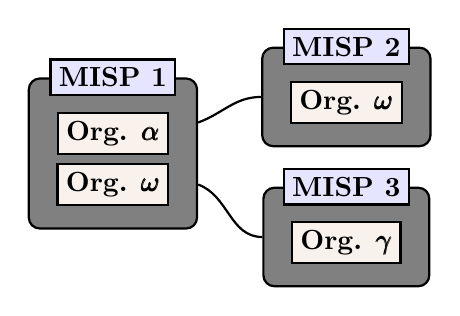
\begin{tikzpicture}[
        node/.style={inner sep=0pt},
        simplebox/.style n args={3}{
            rectangle, rounded corners, thick,
            draw=black, fill=#1,
            minimum width=#2,
            minimum height=#3,
            inner sep=10pt, inner ysep=10pt
        },
        simpleboxtitle/.style = {
            rectangle, rounded corners=0,
            minimum width=1em,
            fill=brown!10, text=black, draw, thick,
            font=\bfseries,
            inner sep=3pt
        },
        header/.style = {%
            inner ysep = +1.0em,
            append after command = {
                \pgfextra{\let\TikZlastnode\tikzlastnode}
                node[simpleboxtitle] (header-\TikZlastnode) at (\TikZlastnode.north) {#1}
            }
        },
        coloredHeader/.style n args={2}{
            inner ysep = +1.0em,
            append after command = {
                \pgfextra{\let\TikZlastnode\tikzlastnode}
                node[simpleboxtitle,fill=#2] (header-\TikZlastnode) at (\TikZlastnode.north) {#1}
            }
        }
    ]

        \node[simpleboxtitle] (orgs01) [] {Org. $\pmb{\alpha}$};
        \node[simpleboxtitle] (orgs02) [below = 0.3em of orgs01] {Org. $\pmb{\omega}$};
        \node[fit = (orgs01) (orgs02)] (orgs0) {};
        \node[simpleboxtitle] (orgs1) [above right= -0.8em and 4em of orgs0] {Org. $\pmb{\omega}$};
        \node[simpleboxtitle] (orgs2) [below = 3.5em of orgs1] {Org. $\pmb{\gamma}$};
        \begin{scope}[on background layer]
            \node[yshift=2pt, fit = (orgs01) (orgs02), simplebox={gray}{1em}{2em}, coloredHeader={MISP 1}{blue!10}] (m1) {};
            \node[yshift=2pt, fit = (orgs1), simplebox={gray}{1em}{2em}, coloredHeader={MISP 2}{blue!10}] (m2) {};
            \node[yshift=2pt, fit = (orgs2), simplebox={gray}{1em}{2em},  coloredHeader={MISP 3}{blue!10}] (m3) {};
        \end{scope}

        \draw[-, thick] (m1) to[out=20, in=180] (m2);
        \draw[-, thick] (m1) to[out=-20, in=180] (m3);
    \end{tikzpicture}
    \end{center}
    \end{multicols*}
}
\cheatboxlarge[The act of \textbf{sharing} where everyone can be a consumer and/or a producer.]{Synchronisation}{

    \vspace*{0.3em}
    A one way synchronisation link between two MISP instances. Organisation $\alpha$ created a \textit{sync user} \faicon{user-plus} on MISP 2 and noted down the generated API Key. A synchronisation link can be created on MISP 1 using the API Key and the organisation of the \textit{sync user}. At that point, MISP 1 can \textit{pull} data from MISP 2 and \textit{push} data to MISP 2.

    \begin{center}
    \pgfdeclarelayer{bg0}    % declare background layer
    \pgfdeclarelayer{bg1}    % declare background layer
    \pgfsetlayers{bg0,bg1,main}  % set the order of the layers (main is the standard layer)
    \begin{tikzpicture}[
        simplebox/.style n args={3}{
            rectangle, rounded corners, thick,
            draw=black, fill=#1,
            minimum width=#2,
            minimum height=#3,
            inner sep=10pt, inner ysep=10pt
        },
        simpleboxtitle/.style = {
            rectangle, rounded corners=0,
            minimum width=1em,
            fill=brown!10, text=black, draw, thick,
            font=\bfseries,
            inner sep=3pt
        },
        header/.style = {%
            inner ysep = +1.0em,
            append after command = {
                \pgfextra{\let\TikZlastnode\tikzlastnode}
                node[simpleboxtitle] (header-\TikZlastnode) at (\TikZlastnode.north) {#1}
            }
        },
        coloredHeader/.style n args={2}{
            inner ysep = +1.0em,
            append after command = {
                \pgfextra{\let\TikZlastnode\tikzlastnode}
                node[simpleboxtitle,fill=#2] (header-\TikZlastnode) at (\TikZlastnode.north) {#1}
            }
        },
        user/.style = {
            inner sep=0pt
        },
        legend/.style = {
            rectangle, rounded corners=0,
            inner sep=2pt,
            draw=black
        },
        nodes = {align = center}
    ]

        \node[user] (misp1users) {\faicon{user} \faicon{user} \faicon{user}};
        \node[user] (misp2users) [right= 13em of misp1users] {\faicon{user} \faicon{user}};
        \node[user] (misp2users2) [right= 3em of misp2users] {\faicon{user} \faicon{user} \faicon{user}};
        \node[user,inner xsep=3pt] (syncuser) [left= 0.0em of misp2users] {\faicon{user-plus}};
        \begin{pgfonlayer}{bg1}
            \node[yshift=2pt, fit = (misp1users), simplebox={white}{1em}{2em}, header = Org. $\pmb{\alpha}$] (misp1org) {};
            \node[yshift=2pt, fit = (misp2users) (syncuser), simplebox={white}{1em}{2em}, header = Org. $\pmb{\alpha}$] (misp2org) {};
            \node[yshift=2pt, fit = (misp2users2), simplebox={gray!30}{1em}{2em}, header = Org. $\pmb{\omega}$] (misp2org2) {};
        \end{pgfonlayer}
        \begin{pgfonlayer}{bg0}
            \node[yshift=+0.5em, fit = (misp1org), simplebox={gray}{11em}{6em}, coloredHeader={MISP 1}{blue!10}] (m1) {};
            \node[yshift=+0.5em, fit = (misp2org) (misp2org2), simplebox={gray}{11em}{6em}, coloredHeader={MISP 2}{blue!10}] (m2) {};
        \end{pgfonlayer}
        \draw[-,very thick] (m1.south) -- ++(0,-15pt) -| ($(syncuser.south) + (0,-2pt)$) node [
            pos=0.25,above,yshift=-0.9em
        ] (textsync) {Sync. connection};
        \def \offsetY {3}
        \draw[->,thick] ($(m1.east) + (1pt,\offsetY pt)$) -- ($(m2.west) + (-1pt,\offsetY pt)$) node [above,midway,yshift=-\offsetY pt] {PUSH};
        \draw[<-,thick] ($(m1.east) + (1pt,-\offsetY pt)$) -- ($(m2.west) + (-1pt,-\offsetY pt)$) node [below,midway,yshift=\offsetY pt] {PULL};
    \end{tikzpicture}
    \end{center}
}
\end{multicols*}
\newpage

\begin{center}{
    \huge{\textbf{MISP Data Model Cheat Sheet}}}\\
\end{center}

\begin{multicols*}{3}
    \begin{minipage}{0.3\textwidth}
        \begin{itemize}[noitemsep,topsep=2pt,parsep=0pt,partopsep=0pt]
            \item[\taggable] Context such as \taxonomies or \clusters can be attached to the element
            \item[\distributable] Can have a distribution level 
            \item[\synchronisable] Can be synchronised to/from other instances
        \end{itemize}
    \end{minipage}
    \vspace*{0.5em}

    % EVENT 
    \cheatbox[\faicon{envelope}]
        [Group datapoints and contexts together. Acting as an envelop, it allows setting its distribution and sharing rules.]
        [Encode incidents, events, reports, …]
        [\taggable \distributable \synchronisable]
        [Encapsulations for contextually linked information.]
        {Event}
        {
            $\blacktriangleright$ \events can contain other elements such as \attributes, \objects and \eventreports.\\
            $\blacktriangleright$ The distribution level and any context added on an \event (such as \taxonomies) are propagated to its underlying data.
        }

    % ATTRIBUTE 
    \cheatbox[\faicon{cube}]
        [Individual data point. Can be an indicator or supporting data.]
        [Domain, IP, link, sha1, attachment, …]
        [\taggable \distributable \synchronisable]
        [Basic building block to share information.]
        {Attribute}
        {
            $\blacktriangleright$ \attributes cannot be duplicated inside the same \event and can have \sightings.\\
            $\blacktriangleright$ The difference between an IoC or supporting data is usualy indicated by the state of the attribute's \texttt{to\_ids} flag.
        }

    % Object 
    \cheatbox[\faicon{cubes}]
        [Groups \attributes that are intrinsically linked together.]
        [File, person, credit-card, x509, device, …]
        [\distributable \synchronisable]
        [Advanced building block providing \attribute compositions via templates.]
        {MISP Object}
        {
            $\blacktriangleright$ \objects have their attribute compositions described in their respective template. They are instanciated with \attributes and can reference \reference other \attributes or \objects.\\
            $\blacktriangleright$ MISP is not required to know the template to save and display the object. However, \textit{edits} will not be possible as the template to validate against is not known.
        }
    \columnbreak

    % Object Reference
    \cheatbox[$\nearrow$]
        [Allows to create relationships between entities, thus creating a graph where they are the edges and entities are the nodes]
        [Represent behaviours, similarities, affiliation, …]
        [\synchronisable]
        [Relationships between individual building blocks.]
        {Object Reference}
        {
            $\blacktriangleright$ \references can have a textual relationship which can come from MISP or be set freely.
        }

    % Sightings
    \cheatbox[\faicon{eye}]
        [Allows to add temporality to the data]
        [Record activity or occurence, perform IoC expiration, …]
        [\synchronisable]
        [Means to convey that a data point has been seen.]
        {Sightings}
        {
            $\blacktriangleright$ \sightings are the best way to express that something has been seen. They can also be used to mark \textit{false positives}.
        }

    % Event report
    \cheatbox[\faicon{file-text}]
        [Supporting data point to describe events or processes]
        [Encode reports, provide more information about the \event, …]
        [\distributable \synchronisable]
        [Advanced building block that can contain text.]
        {Event Report}
        {
            $\blacktriangleright$ \eventreports are markdown-aware and includes a special syntax to reference data points or context.
        }

    % Proposals
    \cheatbox[\faicon{comment}]
        [Allow the correction or the creation of \attributes for \events your organisation does not own.]
        [Disable the IDS flag, Correct errors]
        [\synchronisable]
        [Clone of an \attribute containing information about modification to be done.]
        {Proposals}
        {
            $\blacktriangleright$ As \proposals are sync., if the creator organisation is connected to the MISP instance from where the \proposal has been created, it will be able to either \textit{accept} or \textit{discard} it. 
        }
    \columnbreak

    % Taxonomies
    \cheatbox[$\mathcal{T}$]
        [Enable efficent classification globally understood, easing consumption and automation.]
        [TLP, Confidence, Source, Workflows, Event type, …]
        []
        [Machine and human-readable labels standardised on a common set of vocabularies.]
        {Taxonomies}
        {
            $\blacktriangleright$ Even though MISP allows the creation of free-text tags, it's always preferable to use those coming from \taxonomies if they exists.
        }

    % Galaxies
    \cheatbox[\faicon{rebel}]
        [Bundle \clusters by their type to avoid confusing and to ease searches.]
        [Exploit-Kit, Preventive Measure, MITRE ATT\&CK, Tools, Threat-actors, …]
        []
        [Act as a container to group together context described by \clusters by their type.]
        {Galaxies}
        {}

    % Galaxy Clusters
    \cheatbox[\faicon{rebel}]
        [Enable description of complex high-level information for classification.]
        [\texttt{threat-actor="APT 29"}, \texttt{country="germany"}, \texttt{mitre-attack-pattern="Disk Wipe - T1561"}]
        [\distributable \synchronisable]
        [Kownledge base items used as tags with additional complex meta-data aimed for human consumption.]
        {Galaxies Clusters}
        {
            $\blacktriangleright$ \clusters can be seen as an enhanced \taxonomy as they can have meta-data and relationships with other \clusters.\\
            $\blacktriangleright$ Any \clusters can contain the following:
            \begin{itemize}[noitemsep,topsep=2pt,parsep=0pt,partopsep=0pt]
                \item \texttt{Cluster Elements}: Key-Value pair forming the meta-data.
                \begin{itemize}[noitemsep,topsep=2pt,parsep=0pt,partopsep=0pt]
                    \item[Example:] \texttt{Country:LU}, \texttt{Synonym:APT28}, \texttt{Currency:Dollar}, \texttt{refs:https://*}, …
                \end{itemize}
                \item \texttt{Cluster Relations} (\taggable\synchronisable\distributable): Enable the creation of relationships between one or more \clusters.
                \begin{itemize}[noitemsep,topsep=2pt,parsep=0pt,partopsep=0pt]
                    \item[Example:] Threat actor \texttt{X} \texttt{is similar} to threat actor \texttt{Y} with \texttt{high-likelyhood.}
                \end{itemize}
            \end{itemize}
        }
\end{multicols*}
\newpage

\begin{center}{
    \huge{\textbf{MISP User \& Admin Cheat Sheet}}}\\
\end{center}

\NewDocumentCommand{\multicolstitle}{O{black} O{white} m}{
    \begin{minipage}{0.46\textwidth}
        \begin{center}
            \colorbox{#1}{\Large\textcolor{#2}{\textbf{#3}}}
        \end{center}
    \end{minipage}
}

\newcommand{\bashcode}[1]{
    \colorbox{gray!20}{\lstinline[language=bash]|#1|}
}
\newcommand{\clicode}[1]{
    \colorbox{gray!20}{\lstinline[language=bash]|MISP/app/Console/cake #1|}
}
\newcommand{\httpcode}[3][]{\colorbox{gray!20}{#2 \lstinline[]|#3|}
    \colorbox{gray!20}{\lstinline[]|#1|}
}

\newsavebox\codeboxA
\begin{lrbox}{\codeboxA}
    \begin{minipage}{0.46\textwidth}
    \lstset{style=js}
    \begin{lstlisting}
POST /attributes/restSearch
{"value": "1.2.3.%"}\end{lstlisting}
    \end{minipage}
\end{lrbox}

\newsavebox\codeboxB
\begin{lrbox}{\codeboxB}
    \begin{minipage}{0.46\textwidth}
    \lstset{style=js}
    \begin{lstlisting}
POST /attributes/restSearch
{"tags": ["tlp:white", "!tlp:green"]}\end{lstlisting}
    \end{minipage}
\end{lrbox}

\newsavebox\codeboxC
\begin{lrbox}{\codeboxC}
    \begin{minipage}{0.46\textwidth}
    \lstset{style=js}
    \begin{lstlisting}
POST /attributes/restSearch
{"tags": {"AND": ["tlp:green", "Malware"], "NOT": ["%ransomware%"]}}\end{lstlisting}
    \end{minipage}
\end{lrbox}

\newsavebox\codeboxD
\begin{lrbox}{\codeboxD}
    \begin{minipage}{0.405\textwidth}
    \lstset{style=js}
    \begin{lstlisting}
{"timestamp": 1521846000}
{"timestamp": "7d"}
{"timestamp": ["2d", "1h"]}\end{lstlisting}
    \end{minipage}
\end{lrbox}

\newsavebox\codeboxE
\begin{lrbox}{\codeboxE}
    \begin{minipage}{0.46\textwidth}
    \lstset{style=js}
    \begin{lstlisting}
{
    "galaxy.synonyms": "APT29",
    "galaxy.cfr-target-category": "Financial sector"
}\end{lstlisting}
    \end{minipage}
\end{lrbox}

\newsavebox\codeboxF
\begin{lrbox}{\codeboxF}
    \begin{minipage}{0.46\textwidth}
    \lstset{style=js}
    \begin{lstlisting}
/tags/attachTagToObject
{
    "uuid": "[Could be UUID from Event, Attribute, ...]",
    "tag": "tlp:amber"
}\end{lstlisting}
    \end{minipage}
\end{lrbox}

\begin{multicols*}{2}
    \multicolstitle{User}
    \cheatboxlarge{API}{
        \textbf{\texttt{Wildcard} searches:}\\
        \hspace*{0.5em}\usebox\codeboxA\\
        \textbf{\texttt{Or} and \texttt{Negation} searches:}\\
        \hspace*{0.5em}\usebox\codeboxB\\
        \textbf{\texttt{And} and \texttt{Negation} searches:}\\
        \hspace*{0.5em}\usebox\codeboxC\\
        \textbf{\cluster metadata searches:}\\
        \hspace*{0.5em}\usebox\codeboxE\\
        \textbf{Attach tags:}\\
        \hspace*{0.5em}\usebox\codeboxF\\
        \textbf{Timestamps:}
        \begin{description}[noitemsep,topsep=2pt,parsep=0pt,partopsep=0pt]
            \item \texttt{timestamp}: Time of the last modification on the data
            \begin{itemize}[noitemsep,topsep=2pt,parsep=0pt,partopsep=0pt]
                \item Usecase: Get data was modified in the last $t$
                \item E.g.: Last updated data from a feed
            \end{itemize}
            \item \texttt{publish\_timestamp}: Time at which the event was published
            \begin{itemize}[noitemsep,topsep=2pt,parsep=0pt,partopsep=0pt]
                \item Usecase: Get data that arrived in my system since $t$
                \item E.g.: New data from a feed
            \end{itemize}
            \item \texttt{event\_timestamp}: Used in the Attribute scope
                \begin{itemize}[noitemsep,topsep=2pt,parsep=0pt,partopsep=0pt]
                    \item Usecase: Get events modified in the last $t$
                \end{itemize}
            \item Usage
            \begin{itemize}[noitemsep,topsep=2pt,parsep=0pt,partopsep=0pt]
                \item[] \usebox\codeboxD
            \end{itemize}
        \end{description}
    }

    \cheatboxlarge{Tips \& Tricks}{
        \boxentry{Get JSON Representation}{Append \texttt{.json} at any URL to get the content in JSON format. Example: \texttt{/events/view/42.json}}
    }

    \columnbreak
    \multicolstitle{Admin}
    \cheatboxlarge{Reset Password}{
        API: \httpcode[\{"password": "***"\}]{POST}{/users/initiatePasswordReset/[id]}\\
        CLI: \clicode{Password [email] [password]}
    }
    \cheatboxlarge{Reset Bruteforce login protection}{
        CLI: \clicode{Admin clearBruteforce [email]}
    }
    \cheatboxlarge{Upgrade to the latest version}{%
        All in 1-shot: \clicode{Admin updateMISP}\\
        Manually:
        \begin{enumerate}[noitemsep,topsep=2pt,parsep=0pt,partopsep=0pt]
            \item \bashcode{/var/www/MISP}
            \item \bashcode{git pull origin 2.4}
            \item \bashcode{git submodule update --init --recursive}
            \item \clicode{Admin updateJSON}
            \setlength\itemsep{-0.1em}
            \item Check live update progress \texttt{/servers/updateProgress}
        \end{enumerate}
    }
    \cheatboxlarge{Workers}{
        Restart All: \clicode{Admin restartWorkers}\\
        Add: \clicode{Admin startWorker [queue]}\\
        Stop: \clicode{Admin stopWorker [pid]}
    }
    \cheatboxlarge{Settings}{
        Get: \clicode{Admin getSetting [setting]}\\
        Set: \clicode{Admin setSetting [setting] [value]}\\
        Stop: \clicode{Admin stopWorker [pid]}\\
        Base URL: \clicode{Baseurl [baseurl]}
    }
    \cheatboxlarge{Miscalenous}{
        Clean Caches: \clicode{Admin cleanCaches}\\
        Get IPs For User ID: \clicode{Admin UserIP [user_id]}\\
        Get User ID For User IP: \clicode{Admin IPUser [ip]}\\
        Documentation: \texttt{/events/automation}\\
        Logs files location: \texttt{MISP/app/tmp/logs}
    }
\end{multicols*}

\end{document}
